\section{Robot Design}
\subsection{Fusion360 CAD Implementation}
Significant progress has been achieved in the hardware development phase of the Pookie robot. The outer shell design, now at 80\% completion, has been crafted using Fusion360 CAD software, ensuring precise dimensional accuracy and manufacturability. This development phase has focused on creating a structurally sound and aesthetically cohesive external framework.

\begin{figure}[ht]
    \centering
    \captionsetup{justification=centering}
    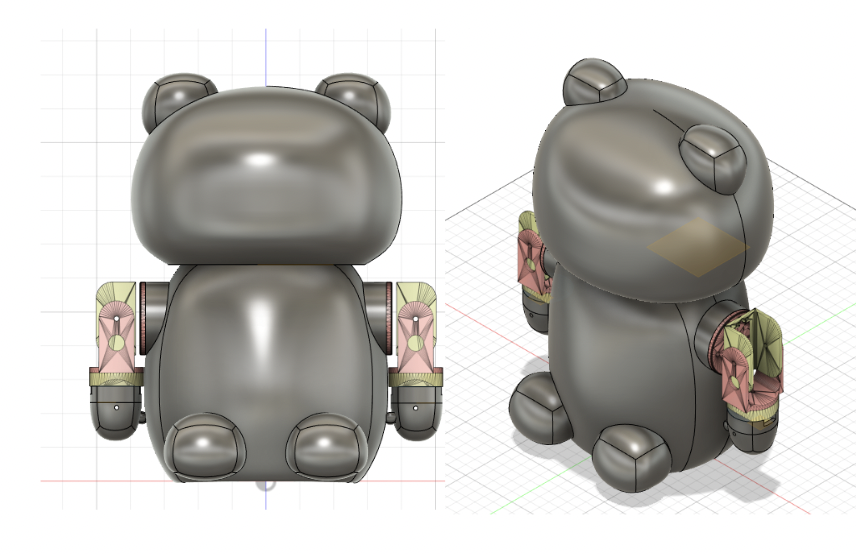
\includegraphics[width=\textwidth]{cad.png}
    \caption{Pookie CAD Implementation}
    \label{fig:cad}
\end{figure}

The robotic arm mechanism represents a completed milestone in the project's development cycle. Through comprehensive mechanical analysis and iterative design refinement, the arm assembly has been successfully engineered to meet all operational requirements. The integration of DS3255 servo motors has been a crucial element in this design phase, with their specifications carefully incorporated to ensure optimal torque delivery and precise movement control.

\begin{figure}[ht]
    \centering
    \captionsetup{justification=centering}
    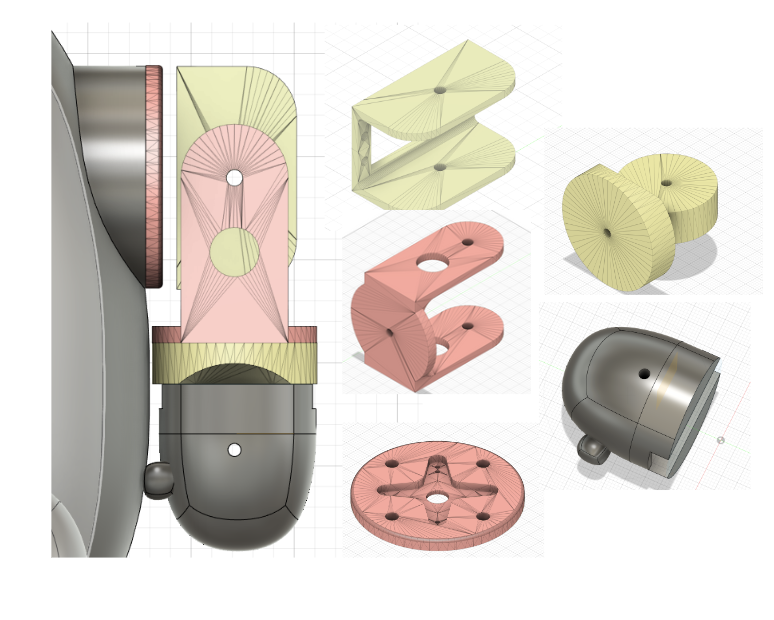
\includegraphics[width=0.7\textwidth]{arm.png}
    \caption{Pookie Robotics Arm Mechanism}
    \label{fig:arm}
\end{figure}

\newpage
The inner shell architecture remains under active development, with significant progress made on critical mechanical components. The servo motor housing for the DS3255 units has been successfully designed in Fusion360, ensuring precise mounting and optimal operational performance. However, the upper head assembly is still in the design phase, requiring further refinement. Concurrent development is underway for the integration frameworks of essential components, including sensor mounting brackets, speaker housings, and LED eye assemblies. This systematic approach to the inner architecture ensures proper component placement while maintaining the structural integrity of the design.

\begin{figure}[ht]
    \centering
    \captionsetup{justification=centering}
    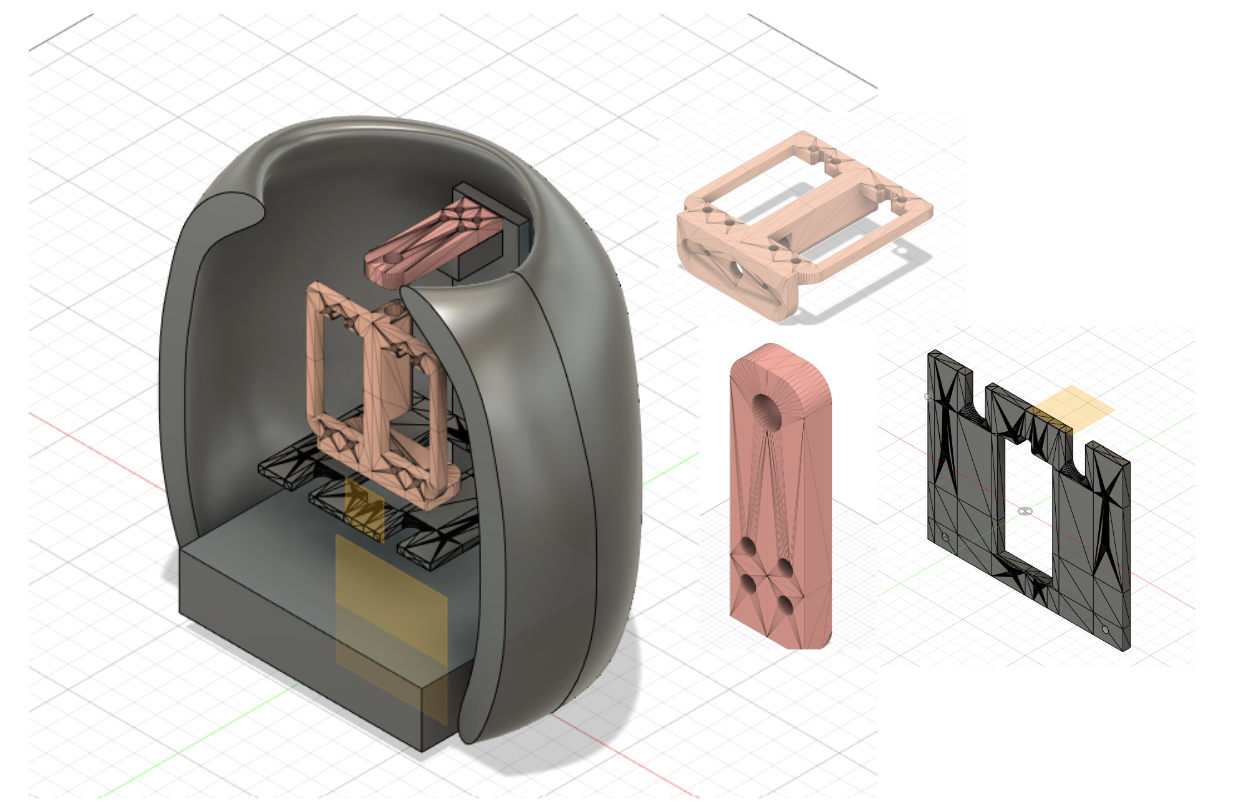
\includegraphics[width=0.7\textwidth]{inner.png}
    \caption{Pookie Inner Shell Design}
    \label{fig:inner}
\end{figure}
